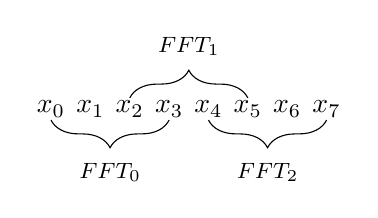
\begin{tikzpicture}
\tikzstyle{box} = [draw,inner sep=7,minimum size=57,line 
width=1, very thick, draw=black, fill=black!20, text width=100, text centered]
\tikzstyle{invisible} = [outer sep=0,inner sep=0,minimum size=0]
\tikzstyle{stealth} = [-stealth, very thick]

\node [] at (-4,0) {$x_0$};
\node [] at (-3.5,0) {$x_1$};
\node [] at (-3,0) {$x_2$};
\node [] at (-2.5,0) {$x_3$};
\node [] at (-2,0) {$x_4$};
\node [] at (-1.5,0) {$x_5$};
\node [] at (-1,0) {$x_6$};
\node [] at (-0.5,0) {$x_7$};

\draw [decorate,decoration={brace,amplitude=10pt,mirror,raise=4pt},yshift=0pt] (-4,0) -- (-2.5,0) node [black,midway,yshift=-0.8cm] {\footnotesize $FFT_0$};
\draw [decorate,decoration={brace,amplitude=10pt,mirror,raise=4pt},yshift=0pt] (-1.5,0) -- (-3,0) node [black,midway,yshift=0.8cm] {\footnotesize $FFT_1$};
\draw [decorate,decoration={brace,amplitude=10pt,mirror,raise=4pt},yshift=0pt] (-2,0) -- (-0.5,0) node [black,midway,yshift=-0.8cm] {\footnotesize $FFT_2$};

\end{tikzpicture}